% Created with jtex v.0.1.6
\documentclass{article}
\usepackage{hyperref}
\usepackage{datetime}
\usepackage{graphicx}
\usepackage{natbib}
\bibliographystyle{abbrvnat}

%%%%%%%%%%%%%%%%%%%%%%%%%%%%%%%%%%%%%%%%%%%%%%%%%%
%%%%%%%%%%%%%%%%%%%%  imports  %%%%%%%%%%%%%%%%%%%
\usepackage{amsmath}
\usepackage{url}
%%%%%%%%%%%%%%%%%%%%%%%%%%%%%%%%%%%%%%%%%%%%%%%%%%

% colors for hyperlinks
\hypersetup{colorlinks=true, allcolors=blue}

\newcommand{\logo}{
  \href{https://curvenote.com}{
\includegraphics[width=2cm]{curvenote.png}}
}

\title{How I Stopped Worrying and Learned to Love Javascript}

\author{riziles}

\newdate{articleDate}{13}{2}{2023}
\date{\displaydate{articleDate}}

\begin{document}
\maketitle
\begin{center}\logo\end{center}


\subsection*{How I Stopped Worrying and Learned to Love Javascript}

So I love \href{https://jupyterbook.org/en/stable/start/your-first-book.html}{Jupyter Book}.
It's a great way to build a beautiful website with Python.
You can add beautiful interactive charts with one of the many plotting libraries supported by Python
such as \href{https://bokeh.org/}{Bokeh} or \href{https://plotly.com/python/}{Plotly}.

But if you want to make things REALLY interactive, you need to add some Javascript.
\href{https://panel.holoviz.org/user_guide/Links.html#defining-javascript-callbacks}{Holoviz Panel}
allows you to embed Javascript callbacks to charts and widgets which
can then be added to Jupyter Book. It's great! I've been experimenting with Panel for a while,
but I ended up learning so much Javascript that I started wondering why I don't just do everything in Javascript.

But then I remembered the beautiful LaTeX PDF documents I created with Jupyter Book,
and decided to stick with Python.

But then I learned about \href{https://myst-tools.org/docs/mystjs}{Myst JS}! And I thought,
what if I build a website in Javascript and used Myst JS to convert it to PDF!?

\subsection*{It Worked!}

\href{%7BassStr%7D/my-document.pdf}{A PDF Version of this page}

\subsection*{Some More Markdown}

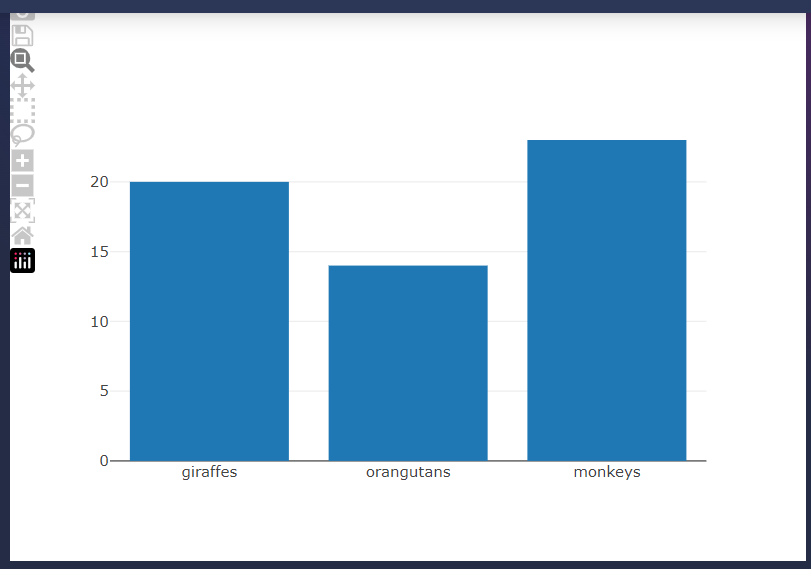
\includegraphics[width=0.7\linewidth]{images/Capture-037f1a6709c029d6e4166b657d95e6ef.PNG}

I can do equations with $\LaTeX$:

\begin{equation}
\frac{x}{x-1} < r_{23}
\end{equation}

Also inline: $x_{i -1}$ So far so good!

What about this Javascript components?

For some reason, inline math doesn't work when passed to a Svelte component using the slot method (\$x+1\$), but double dollar signs do work:

\begin{equation}
x_{i-1}+1 < 5
\end{equation}

Going to try using Mathlifier.
Incidentally, Markdown links don't work inside slots either.

Codeblocks seem to work fine

\begin{verbatim}
import { onMount } from 'svelte';
	
	let headerText;

  export let plotHeader = '';

  export let data = [{
    x: ['giraffes', 'orangutans', 'monkeys'],
    y: [20, 14, 23],
    type: 'bar'
  }];

  onMount(() => {
		headerText = 'A Chart !';
		let plotDiv = document.getElementById('plotDiv');				
		let Plot = new Plotly.newPlot(plotDiv, data, {}, {showSendToCloud:true}); 
  });
\end{verbatim}

\subsection*{Credits}

This website was built with
\href{https://kit.svelte.dev/}{SvelteKit},
\href{https://www.skeleton.dev/}{Skeleton},
\href{https://tailwindcss.com/}{Tailwind},
\href{https://plotly.com/javascript/}{Plotly},
\href{https://mdsvex.pngwn.io/}{MDsveX},
\href{https://github.com/kwshi/rehype-katex-svelte}{rehype-katex-svelte},
\href{https://github.com/remarkjs/remark-math}{remark-math} and
\href{https://github.com/executablebooks/mystjs}{MyST}!


\bibliography{main.bib}
\end{document}
